\subsubsection{Les logs}

Afin que le MJ puisse connaître les actions effectué par les joueurs sans avoir à regarder tout le temps son écran, nous avons implementé une  liste de logs, un historique des actions effectué par les joueurs.

Grâce à cela, le MJ peut surveiller les abus des autres joueurs, pour cela, dans le widget des differents token disponible, un onglet sous la forme d'un accordéon se nomme \og Historique\fg{}, il suffit de cliquer dessus pour faire apparaître les dernière action effectué

\begin{figure}[h!]
    \centering
    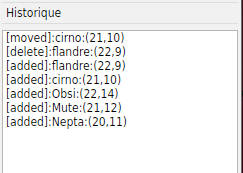
\includegraphics[scale=0.7]{img/log.png}
    \caption{historique}
    \label{fig:log}
\end{figure}